
\documentclass[10pt,letterpaper]{article}

\usepackage[letterpaper,margin=0.70in,headheight=22pt,headsep=16pt,footskip=24pt]{geometry}
\usepackage[T1]{fontenc}
\usepackage[utf8]{inputenc}
\usepackage{lmodern}
\usepackage{microtype}
\usepackage{xcolor}
\usepackage{graphicx}
\usepackage{booktabs}
\usepackage{array}
\usepackage{tabularx}
\usepackage{longtable}
\usepackage{amsmath,amssymb}
\usepackage{tikz}
\usetikzlibrary{arrows.meta,positioning,calc,shapes.geometric,decorations.pathreplacing,fit}
\usepackage{enumitem}
\usepackage{fancyhdr}
\usepackage{titlesec}
\usepackage{caption}
\usepackage{listings}
\usepackage{xurl}
\usepackage[hidelinks]{hyperref}
\usepackage{lastpage}
\usepackage{float}
\usepackage{placeins}

% Generated from wvu_beamer_template/styles/beamercolorthemewvu.sty.
% Standalone copy; no Beamer dependency.
\definecolor{wvu-blue}{HTML}{002855}
\definecolor{wvu-gold}{HTML}{EEAA00}
\definecolor{wvu-star-city-blue}{HTML}{9DDAE6}
\definecolor{wvu-safety-blue}{HTML}{0062A3}
\definecolor{wvu-canary}{HTML}{F7DD63}
\definecolor{wvu-sunset}{HTML}{F58672}
\definecolor{wvu-woodburn}{HTML}{8D4638}
\definecolor{wvu-hemlock}{HTML}{6A724F}
\definecolor{wvu-wild-flour}{HTML}{F2E6C2}
\definecolor{wvu-buckskin}{HTML}{B3A169}
\definecolor{wvu-old-gold}{HTML}{7F6310}
\definecolor{wvu-rattler-gray}{HTML}{554741}
\definecolor{wvu-not-quite-white}{HTML}{F7F7F7}
\definecolor{wvu-coopers-gray}{HTML}{BEB7B3}
\definecolor{wvu-seneca-gray}{HTML}{988E8B}
\definecolor{wvu-coal}{HTML}{1C2B39}

\colorlet{PilotProxyRed}{wvu-woodburn}
\colorlet{PilotProxyGray}{wvu-rattler-gray}
\colorlet{PilotProxyBlue}{wvu-blue}
\colorlet{LightGray}{wvu-not-quite-white}
\colorlet{MidGray}{wvu-coopers-gray}
\colorlet{DarkText}{wvu-coal}
\colorlet{GoodGreen}{wvu-hemlock}
\colorlet{WarnGold}{wvu-old-gold}

\renewcommand{\familydefault}{\sfdefault}
\setlength{\parindent}{0pt}
\setlength{\parskip}{5pt}
\renewcommand{\arraystretch}{1.15}
\sloppy
\setlist[itemize]{leftmargin=1.2em,itemsep=2pt,topsep=2pt}
\setlist[enumerate]{leftmargin=1.4em,itemsep=2pt,topsep=2pt}

\titleformat{\section}{\Large\bfseries\color{DarkText}}{}{0pt}{}[\vspace{-3pt}\color{PilotProxyRed}\titlerule]
\titleformat{\subsection}{\large\bfseries\color{DarkText}}{}{0pt}{}
\titleformat{\subsubsection}{\normalsize\bfseries\color{DarkText}}{}{0pt}{}

\newcommand{\code}[1]{\texttt{\detokenize{#1}}}
\newcommand{\apicode}[1]{\texttt{\detokenize{#1}}}
\newcommand{\yes}{\textcolor{GoodGreen}{Yes}}
\newcommand{\no}{\textcolor{PilotProxyGray}{No}}
\newcolumntype{Y}{>{\raggedright\arraybackslash}X}
\newcolumntype{L}[1]{>{\raggedright\arraybackslash}p{#1}}
\newcolumntype{C}[1]{>{\centering\arraybackslash}p{#1}}
\captionsetup{font=small,labelfont=bf}

\lstdefinestyle{shell}{
  basicstyle=\ttfamily\footnotesize,
  breaklines=true,
  columns=fullflexible,
  frame=single,
  rulecolor=\color{MidGray},
  backgroundcolor=\color{LightGray},
  keepspaces=true,
  showstringspaces=false
}
\lstdefinestyle{cstyle}{
  basicstyle=\ttfamily\footnotesize,
  breaklines=true,
  columns=fullflexible,
  frame=single,
  rulecolor=\color{MidGray},
  backgroundcolor=\color{LightGray},
  keepspaces=true,
  showstringspaces=false
}
\lstset{style=shell}

\newcommand{\notebox}[1]{%
  \vspace{4pt}\noindent\fcolorbox{PilotProxyBlue}{LightGray}{%
  \begin{minipage}{0.965\linewidth}%
  \textbf{Note:} #1%
  \end{minipage}}\vspace{4pt}}

\newcommand{\importantbox}[1]{%
  \vspace{4pt}\noindent\fcolorbox{PilotProxyRed}{LightGray}{%
  \begin{minipage}{0.965\linewidth}%
  \textbf{Important:} #1%
  \end{minipage}}\vspace{4pt}}

\newcommand{\field}[1]{\texttt{\detokenize{#1}}}
\newcommand{\dB}{\,\mathrm{dB}}

% Single-sourced numeric specifications (versions, geometry, null_power_ratio range,
% digests). Regenerate with: python tools/generate_doc_specs.py
\input{generated/specs.tex}

\pagestyle{fancy}
\fancyhf{}
\fancyhead[L]{\small PilotProxy-UG001}
\fancyhead[C]{\small CUDA DTV Pilot Detector}
\fancyhead[R]{\small User Guide}
\fancyfoot[L]{\small PilotProxy-UG001}
\fancyfoot[C]{\small Pilot-informed DTV detector}
\fancyfoot[R]{\small Page \thepage\ of \pageref{LastPage}}
\renewcommand{\headrulewidth}{0.8pt}
\renewcommand{\headrule}{\hbox to\headwidth{\color{PilotProxyRed}\leaders\hrule height \headrulewidth\hfill}}
\renewcommand{\footrulewidth}{0.8pt}
\renewcommand{\footrule}{\hbox to\headwidth{\color{PilotProxyRed}\leaders\hrule height \footrulewidth\hfill}}

\title{PilotProxy CUDA DTV Pilot Detector\\User Guide}
\author{Dylan J. Gormley}
\date{PilotProxy-UG001 \\ October 2026}

\begin{document}
\thispagestyle{empty}
\begin{tikzpicture}[remember picture,overlay]
  \draw[PilotProxyRed,line width=2pt] ($(current page.north west)+(0.72in,-0.35in)$) -- ($(current page.north east)+(-0.72in,-0.35in)$);
  \draw[PilotProxyRed,line width=1pt] ($(current page.south west)+(0.72in,0.45in)$) -- ($(current page.south east)+(-0.72in,0.45in)$);
\end{tikzpicture}
\vspace*{0.25in}
{\fontsize{30}{32}\selectfont\bfseries\color{PilotProxyRed}PilotProxy}\par
\vspace{0.12in}
{\fontsize{23}{26}\selectfont\bfseries CUDA DTV Pilot Detector}\par
\vspace{0.08in}
{\Large User Guide}\par
\vspace{0.35in}
{\large PilotProxy-UG001}\par
{\large October 2026}\par
\vfill
\begin{tabularx}{\linewidth}{|>{\bfseries}L{0.25\linewidth}|Y|}
\hline
Document scope & Package installation, source-tree CUDA build, ATSC waveform generation, detector tests, receiver integration, and interpretation of fixed-point outputs, including the time-coherent fine products.\\ \hline
Package version & \code{pilot-proxy} v\ppPackageVersion; kernel core \ppKernelCoreVersion.\\ \hline
Primary runtime controls & A physical channel or pilot frequency selects weights. Frame size and, for synthetic threshold tests, DTV data-shelf SNR control the detector run.\\ \hline
CHIME/CANFAR mode & The CHIME path masks at $F>\mu_0$, where $\mu_0$ is fixed by the quantized weight norms. It does not use a mean estimated from CANFAR data.\\ \hline
Project affiliation & West Virginia University.\\ \hline
\end{tabularx}
\newpage

\setcounter{tocdepth}{1}
\tableofcontents
\clearpage

\section{Introduction}

PilotProxy measures ATSC 1.0 pilot tones with a fixed-point CUDA local-reference power-ratio detector. We use the narrow pilot as a proxy for a DTV data shelf that may lie below the broadband noise floor. The standalone testbench generates its own waveform and receiver geometry, while the CHIME workflow receives instrument metadata and packed baseband data through its own adapter.

The kernel is kept independent of the instrument by design. It measures target and reference powers with no knowledge of physical channels, decibels, or telescope layout, and host software supplies those meanings and records them with the output.

\subsection{Detector Objective}

\begin{quote}
Given a local ATSC pilot excess, estimate the equivalent ATSC 1.0 data-shelf SNR relative to the stated non-DTV reference floor.
\end{quote}

In this guide, we first build and test the detector. We then generate an ATSC waveform, audit it, add noise at a requested shelf SNR, quantize the samples, and run the detector. Finally, we discuss receiver integration, output fields, limitations, and common failures.

\subsection{Package Contents}

\begin{longtable}{|L{0.30\linewidth}|L{0.62\linewidth}|}
\hline
\textbf{Path} & \textbf{Contents}\\ \hline
\code{cuda/} & CUDA kernel, public C header, CPU reference model, and C/CUDA tests.\\ \hline
\code{src/pilot_proxy/} & Python package for kernel loading, detector geometry, reference channelization, DTV unit conversion, channel helpers, and detection.\\ \hline
\code{src/pilot_proxy/testbench/} & GNU Radio ATSC generation, waveform audit, AWGN injection, quantization, and SNR evaluation.\\ \hline
\code{weights/} & Prebuilt ATSC reference detector weights for channels 14-36.\\ \hline
\code{docs/} & Markdown definitions, data sheet, and user guide source.\\ \hline
\code{examples/quickstart.sh} & End-to-end release sanity-check workflow.\\ \hline
\end{longtable}

\section{Definitions}

The detector compares one target power with two local reference powers. For one result, we compute
\begin{equation}
  F=\frac{2P_t}{P_{r1}+P_{r2}},\qquad Q=F/\mu_0,\qquad e=Q-1.
\end{equation}
The normalization \(\mu_0\) is the ratio of the exact squared norms of the packed target and reference weights. The raw diagnostic \(F-1\) is not the physical excess, which is \(e\). We use \(\mathrm{PNR}_{\mathrm{bin},dB}=10\log_{10}e\) for \(e>0\), and convert it to an equivalent DTV data-shelf SNR with
\begin{equation}
  \mathrm{SNR}_{\mathrm{shelf},dB} = \mathrm{PNR}_{\mathrm{bin},dB}
  -10\log_{10}(B_{\mathrm{DTV}}/B_{\mathrm{bin}})
  +\mathrm{pilot\_below\_data\_db}
  -10\log_{10}(\eta_p).
\end{equation}
For the checked-in reference geometry,
\begin{equation}
  B_{\mathrm{bin}}=\frac{400\,\mathrm{MHz}}{1024\times128}=3051.7578125\,\mathrm{Hz},
\end{equation}
which gives the bandwidth spreading term
\begin{equation}
  10\log_{10}(6\,\mathrm{MHz}/B_{\mathrm{bin}})=32.936\dB.
\end{equation}

\notebox{We independently recomputed this conversion from the checked-in formulas. A 1 dB normalized power-ratio level gives \(Q=1.2589\), \(e=0.2589\), \(\mathrm{PNR}_{\mathrm{bin}}=-5.868\dB\), and \(\mathrm{SNR}_{\mathrm{shelf}}\approx -27.50\dB\) for the 3.052 kHz reference bin.}


\begin{figure}[H]
\centering
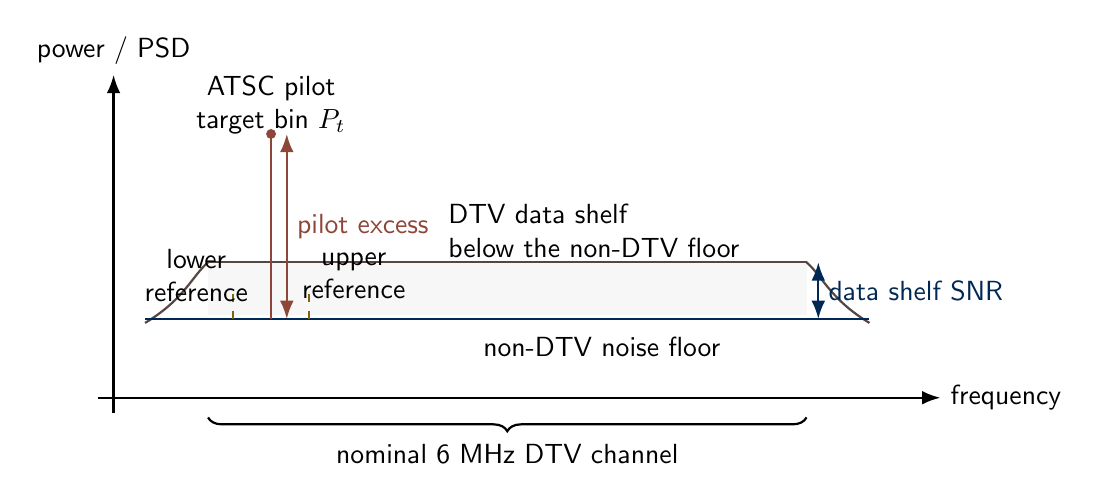
\begin{tikzpicture}[x=1.0cm,y=1.0cm,>=Latex]
  \draw[->,thick] (-0.2,0) -- (10.5,0) node[right]{frequency};
  \draw[->,thick] (0,-0.2) -- (0,4.1) node[above]{power / PSD};
  \draw[fill=LightGray,draw=none] (1.2,1.05) rectangle (8.8,1.72);
  \draw[thick,PilotProxyGray] (1.2,1.72) -- (8.8,1.72);
  \draw[thick,PilotProxyGray] (0.4,0.95) .. controls (0.9,1.25) and (1.0,1.55) .. (1.2,1.72);
  \draw[thick,PilotProxyGray] (8.8,1.72) .. controls (9.0,1.55) and (9.1,1.25) .. (9.6,0.95);
  \draw[thick,PilotProxyBlue] (0.4,1.0) -- (9.6,1.0);
  \draw[thick,PilotProxyRed] (2.0,1.0) -- (2.0,3.35);
  \draw[fill=PilotProxyRed,draw=PilotProxyRed] (2.0,3.35) circle (0.055);
  \draw[dashed,thick,WarnGold] (1.52,1.0) -- (1.52,1.35);
  \draw[dashed,thick,WarnGold] (2.48,1.0) -- (2.48,1.35);
  \draw[<->,thick,PilotProxyRed] (2.20,1.0) -- (2.20,3.35) node[midway,right]{pilot excess};
  \draw[<->,thick,PilotProxyBlue] (8.95,1.0) -- (8.95,1.72) node[midway,right]{data shelf SNR};
  \draw[decorate,decoration={brace,mirror,amplitude=5pt},thick] (1.2,-0.25) -- (8.8,-0.25)
    node[midway,below=6pt]{nominal 6 MHz DTV channel};
  \node[align=center] at (2.0,3.72) {ATSC pilot\\target bin $P_t$};
  \node[align=center] at (1.05,1.55) {lower\\reference};
  \node[align=center] at (3.05,1.55) {upper\\reference};
  \node[align=left] at (6.1,2.12) {DTV data shelf\\below the non-DTV floor};
  \node[align=left] at (6.2,0.65) {non-DTV noise floor};
\end{tikzpicture}
\caption{Signal definitions used by the detector. The red line is the ATSC pilot in the target bin \(P_t\), the gold dashed lines mark the lower and upper reference bins, the gray band is the DTV data shelf, and the blue line is the non-DTV noise floor. The kernel compares the target bin with the two reference bins, and host software converts the resulting one-bin excess to an equivalent 6 MHz data-shelf SNR under the recorded calibration constants.}
\label{fig:spectrum_definitions}
\end{figure}


\section{Installation Model}

The end-to-end workflows in this guide use an editable checkout, with the extras required by each workflow:
\begin{lstlisting}[style=shell]
python -m pip install -e ".[test]"              # CPU-side tests
python -m pip install -e ".[cuda,test,plot]"    # CUDA and plots
pilot-proxy --help
\end{lstlisting}
Built wheels and source distributions contain the reference weight bank and the \code{configs/} tree, so default-resource CPU commands such as \code{list-channels} can run from any directory. The examples, the repository-relative generated paths, the helper scripts, and the two-interpreter workflows that use subprocesses are run from a checkout or given explicit paths. The CUDA shared library is not part of the Python distribution and is built from a clone before any GPU-backed command runs.

\subsection{Python Environments}

When GNU Radio is installed as a system package, two Python interpreters may be necessary:
\begin{itemize}
  \item GNU Radio Python: used for ATSC generation and GNU Radio AWGN, typically \code{/usr/bin/python3}.
  \item CUDA Python: the repository virtual environment, installed with the \code{cuda} and \code{test} extras and, when needed, the \code{plot} extra, and used for CuPy, the CUDA shared library, and detector evaluation.
\end{itemize}

The CUDA environment stays active for the examples below. The \code{generate-atsc} command and the GNU Radio noise source invoke the interpreter supplied through \code{--gnuradio-python}, typically \code{/usr/bin/python3}, and PilotProxy must also be importable by that interpreter. This guide supports an editable source checkout, whose wrapper supplies the \code{src/} path of the checkout to the child process. With a wheel, PilotProxy must be installed for the GNU Radio interpreter or reached through an explicit compatible \code{PYTHONPATH}, since an installation in the CUDA environment alone is not visible to that interpreter. On WSL, the CUDA driver path is commonly \code{/usr/lib/wsl/lib}, and it is verified on the target host.

On WSL, adding the Python environment's \code{lib/} directory to
\code{LD_LIBRARY_PATH} can make \code{/usr/bin/bash} load that environment's
\code{libtinfo.so.6} and print a \code{no version information available}
warning. The examples require only the CUDA driver path. When user-site packages shadow the NumPy build used by GNU Radio, \code{--no-python-user-site} is passed to \code{generate-atsc}. The GNU Radio noise subprocess of the evaluator already disables the user site.

\section{Build and Test}

\subsection{Build the CUDA Kernel}

The kernel is built for the target GPU architecture with:
\begin{lstlisting}[style=shell]
make build-kernel   # SM auto-detected; pass SM=<arch> to override
\end{lstlisting}
This builds \code{cuda/libpilotproxy.so} and stages a copy to:
\begin{lstlisting}[style=shell]
~/.cache/pilot_proxy/libpilotproxy.so
\end{lstlisting}
On WSL, the cached copy avoids loading the shared library directly from \code{/mnt/c}. After a rebuild under \code{cuda/} alone, the staged copy is removed with:
\begin{lstlisting}[style=shell]
make clean-cache
\end{lstlisting}

\subsection{Run Tests}

The Python tests are run with:
\begin{lstlisting}[style=shell]
python -m pytest tests -q
\end{lstlisting}
The CUDA and kernel tests are run on a CUDA-capable host with:
\begin{lstlisting}[style=shell]
make -C cuda test DP4A=1   # SM auto-detected
\end{lstlisting}
The Python, CPU, CUDA, and GNU Radio checks are run as distinct suites, and the commit, host, and commands are recorded for each release test. A Python-only result says nothing about CUDA or GNU Radio behavior, so those checks are run on a suitable target before a release is tagged.

\section{Quickstart}

The provided script exercises the main standalone path:
\begin{lstlisting}[style=shell]
bash examples/quickstart.sh   # GPU architecture auto-detected
\end{lstlisting}
The output has a waveform audit, the detector-input generation, an SNR evaluation, and the detection JSON. The summary headings are shown below. Numeric rows are not reproduced here, since the result is the output recorded when the script is rerun on the target commit.
\begin{lstlisting}[style=shell]
frequency_offset_hz, requested_data_shelf_snr_db,
measured_truth_data_shelf_snr_db, cpu_float_estimated_data_shelf_snr_db,
gpu_estimated_data_shelf_snr_db, gpu_snr_error_db
...
blocks, positive_excess_set, coarse_power_ratio_mean,
estimated_data_shelf_snr_db_mean
...
\end{lstlisting}

\section{Generate and Audit an ATSC Waveform}

\subsection{Generate a Reference ATSC Signal}

The reference ATSC waveform is generated under the GNU Radio interpreter given by \code{--gnuradio-python}:
\begin{lstlisting}[style=shell]
pilot-proxy generate-atsc \
  --gnuradio-python /usr/bin/python3 \
  --output-iq generated/atsc/atsc_8vsb_complex64.cfile \
  --num-iq-samples 600000
\end{lstlisting}

\subsection{Audit the Reference Waveform}

The generated waveform is audited before detector evaluation:
\begin{lstlisting}[style=shell]
pilot-proxy audit-atsc \
  --input-iq generated/atsc/atsc_8vsb_complex64.cfile
\end{lstlisting}
The audit records the pilot frequency, pilot-to-data power, occupied bandwidth, shelf flatness, and edge rolloff. The field \field{measured_pilot_to_data_power_db} is the signed quantity \(10\log_{10}(P_{\mathrm{pilot}}/P_{\mathrm{data}})\). The field \field{measured_pilot_below_data_db} records its positive magnitude when the pilot is below the data shelf.

\notebox{The audit reports pilot frequency in the generated complex-baseband coordinate. For physical channel 14, the baseband pilot corresponds to an RF pilot at 470.309441 MHz after reference-band placement.}

\section{Reference Channelizer and Detector Resolution}

The standalone testbench uses the following polyphase filter-bank (PFB) reference front end:
\begin{longtable}{|L{0.36\linewidth}|L{0.56\linewidth}|}
\hline
\textbf{Quantity} & \textbf{Value}\\ \hline
Real ADC sample rate & 800 MS/s \\ \hline
Reference lower band edge & 400 MHz \\ \hline
Reference bandwidth & 400 MHz \\ \hline
PFB taps & 4 \\ \hline
PFB FFT size & 2048 real-input samples \\ \hline
Usable positive-frequency channels & 1024 \\ \hline
Coarse-channel spacing & 390.625 kHz \\ \hline
Detector window & \ppDetectorWindowSamples\ samples \\ \hline
Detector-bin width & \ppDetectorBinHz\ Hz \\ \hline
Fine-bin width (padded) & \ppFineBinHz\ Hz (\ppFineNumBins\ bins per detector bin span) \\ \hline
\end{longtable}
This geometry gives a detector-bin width of \ppDetectorBinHz\ Hz. The default pilot-to-shelf conversion is valid for this geometry only, and another receiver must supply its measured or modeled effective noise bandwidth. In this guide, the \ppDetectorBinHz\ Hz resolution set by the \(K=\ppDetectorWindowSamples\) window is known as the \emph{detector bin}, and the \ppFineBinHz\ Hz resolution of the padded window-axis FFT described in Section~\ref{sec:fineproducts} is known as the \emph{fine bin}.

\section{Channel Selection}

The physical channels supported by the shipped weight bank are listed with:
\begin{lstlisting}[style=shell]
pilot-proxy list-channels
\end{lstlisting}
The shipped weights cover physical channels 14 through 36. The frequency helpers accept other UHF channels, but the detector still requires a matching row in the weight manifest. In the standalone reference coordinate, which ascends in frequency, channels 14, 21, and 36 are at coarse indices 179, 287, and 517. The shipped CHIME manifest, in the post-Nyquist-zone-normalization coordinate reported by \code{list-channels}, stores the same targets at 843, 735, and 505. An index is therefore compared with another only when both name their coordinate system.

The default channel is physical channel 14:
\begin{equation}
  f_{\mathrm{lower}}=470\,\mathrm{MHz},\quad f_{\mathrm{pilot}}=470.309441\,\mathrm{MHz},\quad f_{\mathrm{center}}=473\,\mathrm{MHz}.
\end{equation}
In the shipped DC-centered bank, physical channel 14 tests a coarse-channel boundary. Its weight row wraps the lower reference across the circular coarse-channel spectrum while preserving the requested \(-2,+2\) detector-bin offsets. The manifest records this choice with \field{adaptive_reference_placement=true}, and \code{list-channels} prints the corresponding placement \code{NOTE}. No shipped channel collides with, or shifts around, the forbidden coarse-channel DC tone.

\section{Quantize and Create Detector Input}

A packed detector matrix is created with:
\begin{lstlisting}[style=shell]
pilot-proxy quantize \
  --input-iq generated/atsc/atsc_8vsb_complex64.cfile \
  --physical-channel 14 \
  --frame-size-samples 16384
\end{lstlisting}
This example uses a 16384-sample frame, the frame of the checked-in CHIME
reference profile. In an integration, the frame size is matched to the frame of
the correlator, and it must be a positive multiple of the selected detector
window. The detector core supports \(K=64\) and \(K=128\). The CHIME profile
selects \(K=128\), while the CHORD profiles select \(K=64\). This repository is
designed for the CHIME F-engine upgrade target of \(2^{14}=16384\) samples, and
this value makes no statement about the CHIME correlator deployed today. Since
the software infers no universal frame size from HDF5 metadata,
\code{chime-run --frame-size-samples} is set from verified product information,
and the Pilot Proxy CHIME instrument \code{nfft} used by \code{chime-scan} is
set from the same information. The resolved value is recorded with each
real-data product.

The output matrix is row-major and has shape \code{(rows, K)} or
\code{(batch, rows, K)} with dtype \code{int8}, where \code{K} is the selected
compiled detector window. The CUDA wrapper checks both properties before
passing pointers to the kernel.

\section{Evaluate Shelf-SNR Response}

The synthetic evaluator is run with the CUDA backend, here with the WSL driver path:
\begin{lstlisting}[style=shell]
LD_LIBRARY_PATH=/usr/lib/wsl/lib \
pilot-proxy evaluate-snr \
  --input-iq generated/atsc/atsc_8vsb_complex64.cfile \
  --physical-channel 14 \
  --frame-size-samples 16384 \
  --requested-data-shelf-snr-db -26 \
  --threshold-data-shelf-snr-db -26 \
  --noise-trials 10 \
  --noise-source gnuradio \
  --gnuradio-python /usr/bin/python3
\end{lstlisting}
Outputs are written under \code{generated/dtv_snr_eval/}:
\begin{itemize}
  \item \code{dtv_snr_eval.csv}: per-trial validation rows;
  \item \code{dtv_snr_summary.csv}: grouped summary;
  \item \code{dtv_snr_eval.json}: full strict-JSON validation report.
\end{itemize}

If neither explicit \code{--requested-data-shelf-snr-db} values nor an
\code{--snr-start-db}/\code{--snr-stop-db}/\code{--snr-step-db} range is
provided, the evaluator sweeps from \(-60\dB\) to \(0\dB\) in 3 dB steps.
Each trial counted by \code{--noise-trials} adds one independently generated
noise frame at every requested SNR and frequency offset, so a response curve
needs several trials per point. The GNU Radio noise path exercises more of the
reference signal chain, while the Python noise path reduces the runtime of a
large sweep:
\begin{lstlisting}[style=shell]
LD_LIBRARY_PATH=/usr/lib/wsl/lib \
pilot-proxy evaluate-snr \
  --input-iq generated/atsc/atsc_8vsb_complex64.cfile \
  --physical-channel 14 \
  --frame-size-samples 16384 \
  --num-input-streams 1 \
  --threshold-data-shelf-snr-db -26 \
  --noise-trials 10 \
  --noise-source python
\end{lstlisting}
This configuration produces 210 detector frames, with 10 frames at each of 21
SNR values. Ten trials are enough to check the workflow, but they do not support
an uncertainty claim in a publication. The final trial count is chosen from the
precision required for the plotted interval, and that choice is recorded. When
the \(-1\mathrm{kHz}\), \(0\mathrm{Hz}\), and \(+1\mathrm{kHz}\) curves are
needed, \code{--standard-frequency-offset-sweep} triples the number of evaluated
offset conditions.

Large sweeps require no GPU. With \code{--detector-backend cpu-reference}, the primary fields come from the integer CPU reference, and each row records the backend. Before a CPU-only sweep is taken as representative of the CUDA implementation, a small sample with the same seed is compared on both backends, for example with:
\begin{lstlisting}[style=shell]
pilot-proxy evaluate-snr \
  --input-iq generated/atsc/atsc_8vsb_complex64.cfile \
  --physical-channel 14 \
  --frame-size-samples 16384 \
  --num-input-streams 1 \
  --threshold-data-shelf-snr-db -26 \
  --noise-trials 300 \
  --noise-source python \
  --detector-backend cpu-reference
\end{lstlisting}

For a CUDA-backed sweep, the grouped result is rendered without plot smoothing:
\begin{lstlisting}[style=shell]
pilot-proxy plot-results
\end{lstlisting}
The CSV, JSON, and PNG use the same grouped summary values. The plot helper labels its selected fixed-point series ``GPU fixed-point'' in every case. For a \code{cpu-reference} result that label is wrong, so the CSV is plotted directly or the series is relabeled ``CPU fixed-point,'' and the recorded \field{detector_backend} is kept with the figure.

\begin{figure}[H]
\centering
\IfFileExists{../generated/dtv_snr_eval/dtv_snr_sweep.png}{%
\includegraphics[width=0.92\linewidth]{../generated/dtv_snr_eval/dtv_snr_sweep.png}
\caption{Example shelf-SNR response for the synthetic configuration of this section, from \(-60\dB\) to \(0\dB\) in 3 dB steps, with 10 Python-noise trials per point, one input stream, and no smoothing. The diagonal marks equal input and output SNR. The two curves are the unquantized floating-point model and the selected packed-int4 fixed-point backend. Ten trials per point demonstrate the workflow and do not set the uncertainty of a publication result.}
}{%
\fbox{\parbox{0.86\linewidth}{\centering The optional generated SNR sweep figure was not found. The validation sweep and plot workflow create \code{generated/dtv_snr_eval/dtv_snr_sweep.png}.}}
\caption{Example shelf-SNR response for the synthetic configuration of this section, from \(-60\dB\) to \(0\dB\) in 3 dB steps, with 10 Python-noise trials per point, one input stream, and no smoothing. The diagonal marks equal input and output SNR. The two curves are the unquantized floating-point model and the selected packed-int4 fixed-point backend. Ten trials per point demonstrate the workflow and do not set the uncertainty of a publication result.}
}
\label{fig:snr_sweep_10trial}
\end{figure}

The main report fields are:
\begin{itemize}
  \item \field{requested_data_shelf_snr_db}
  \item \field{measured_truth_data_shelf_snr_db}
  \item \field{measured_truth_composite_atsc_snr_db}
  \item \field{p_target_u64}, \field{p_ref_lower_u64}, \field{p_ref_upper_u64}
  \item \field{coarse_power_ratio}, \field{normalized_coarse_power_ratio_db}, \field{raw_pilot_excess}, \field{pilot_excess_db}
  \item \field{estimated_data_shelf_snr_db}, \field{snr_error_db}
  \item \field{mask}, when \code{--threshold-data-shelf-snr-db} is supplied.
\end{itemize}


\begin{figure}[H]
\centering
% Standalone validation flow.
% This file is the one source of the diagram. It is \input by PilotProxy_DS001
% (Data Sheet) and PilotProxy_UG001 (User Guide) and rendered to
% validation_flow.svg for docs/USAGE.md. It needs the tikz libraries
% arrows.meta and positioning, and the colors PilotProxyBlue (WVU blue) and
% LightGray (WVU not-quite-white) defined by the host document, or by
% validation_flow_standalone.tex when the svg is rendered. The svg must be
% rendered again after each edit:
%   cd docs/figures && pdflatex validation_flow_standalone.tex \
%     && pdftocairo -svg validation_flow_standalone.pdf validation_flow.svg
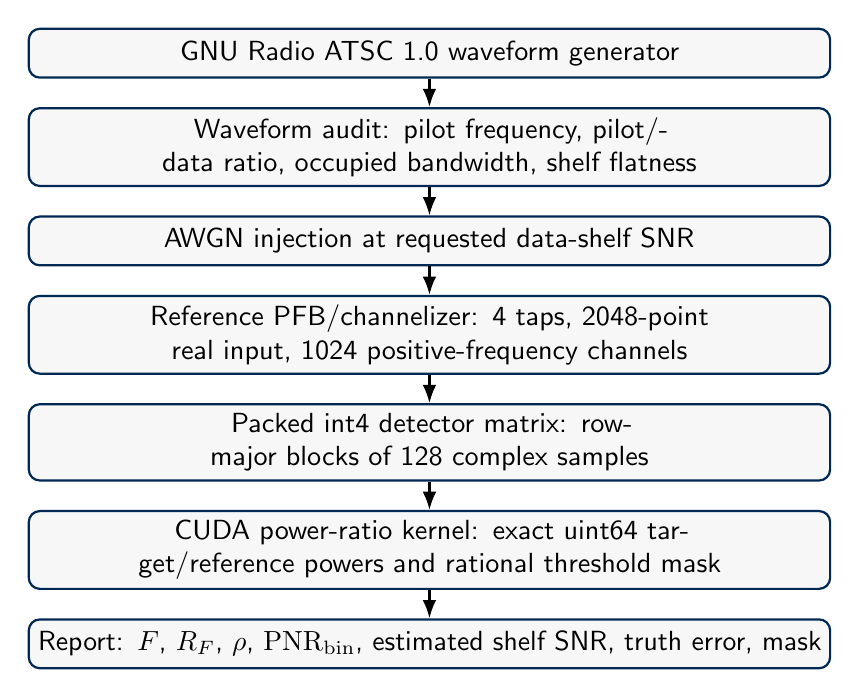
\begin{tikzpicture}[node distance=0.36cm,>=Latex]
\tikzstyle{block}=[rectangle,rounded corners,draw=PilotProxyBlue,thick,fill=LightGray,minimum height=0.62cm,text width=0.82\linewidth,align=center]
\node[block] (a) {GNU Radio ATSC 1.0 waveform generator};
\node[block,below=of a] (b) {Waveform audit: pilot frequency, pilot/data ratio, occupied bandwidth, shelf flatness};
\node[block,below=of b] (c) {AWGN injection at requested data-shelf SNR};
\node[block,below=of c] (d) {Reference PFB/channelizer: 4 taps, 2048-point real input, 1024 positive-frequency channels};
\node[block,below=of d] (e) {Packed int4 detector matrix: row-major blocks of 128 complex samples};
\node[block,below=of e] (f) {CUDA power-ratio kernel: exact uint64 target/reference powers and rational threshold mask};
\node[block,below=of f] (g) {Report: $F$, $R_F$, $\rho$, $\mathrm{PNR}_{\mathrm{bin}}$, estimated shelf SNR, truth error, mask};
\draw[->,thick] (a) -- (b);
\draw[->,thick] (b) -- (c);
\draw[->,thick] (c) -- (d);
\draw[->,thick] (d) -- (e);
\draw[->,thick] (e) -- (f);
\draw[->,thick] (f) -- (g);
\end{tikzpicture}

\caption{Standalone validation flow. The included reference front end converts a generated ATSC waveform into the packed-input contract used by the detector.}
\label{fig:validation_flow}
\end{figure}


\newpage\section{Detection on a Packed Matrix}

Detection on a prebuilt packed detector matrix is run with:
\begin{lstlisting}[style=shell]
LD_LIBRARY_PATH=/usr/lib/wsl/lib \
pilot-proxy detect \
  --input-detector-matrix generated/detector_input/detector_matrix_i4.npy
\end{lstlisting}
The command reads the pilot identity from the \code{metadata.json} sidecar that
\code{quantize} writes next to the matrix, and an explicit
\code{--physical-channel} or \code{--dtv-pilot-mhz} must agree with it. With
neither a sidecar nor a flag, \code{detect} stops, because it cannot select a
weight row safely. If \code{detector_matrix_i4.npy} is absent but the batched
\code{detector_blocks_i4.npy} file exists, \code{detect} resolves the default
input to the batched file. If neither file exists, \code{quantize} must be run
first.

The detector JSON contains:
\begin{itemize}
  \item \field{selected_weight_layout}
  \item \field{result_schema} with \code{schema_version=pilotproxy_result_schema_v2}
  \item \field{layout} with \field{frame_size_samples}, \field{num_input_streams}, \field{windows_per_stream}, and \field{detector_rows_per_frame}
  \item \field{mask_rule}, \field{target_norm_sq}, \field{reference_norm_sum_sq}, and \field{null_power_ratio}
  \item per-block \field{mask} and \field{normalized_positive_excess_mask}, exact powers, \field{coarse_power_ratio}, raw \field{raw_pilot_excess}, norm-corrected \field{normalized_pilot_excess}, and estimated shelf SNR.
\end{itemize}
The \code{detect} command applies no user-supplied shelf-SNR threshold. Its threshold fields in \field{result_schema} are \code{null}, and it masks a valid block at the norm-corrected condition \(F>\mu_0\). The basic raw convention \(F>1\) is used to define \(\rho=F-1\), while the CHIME mask rule is \(F>\mu_0\).

\section{Receiver Integration Contract}

The kernel does not encode telescope metadata. Receiver integrations provide the following JSON records and arrays:
\begin{itemize}
  \item \code{configs/detector_core/pilotproxy_cuda_local_reference_power_ratio.json} describes the locked CUDA kernel contract.
  \item \code{receiver_profile.json} describes RF band, channelizer geometry, Nyquist zone, frame size, input streams, quantization defaults, bin ENBW, and pilot-capture efficiency.
  \item \code{stream_map.json} maps stream indices to feed, polarization, beam, or other receiver-specific labels.
  \item \code{check-profile}, \code{check-layout}, \code{make-weights}, and \code{chime-run} consume the applicable profile or stream-map records. The standalone \code{detect} command selects shipped weights from its sidecar or channel flag, while \code{evaluate-snr} uses the fixed testbench geometry.
\end{itemize}

\begin{figure}[H]
\centering
% Shared diagram of the implemented Kotekan mask path. Requires arrows.meta,
% positioning, calc and the PilotProxy color names from the host document.
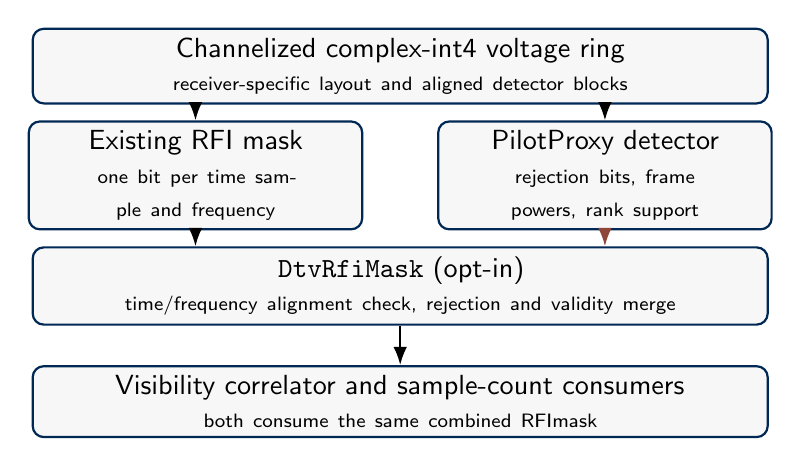
\begin{tikzpicture}[node distance=0.5cm,>=Latex,
  blk/.style={rectangle,rounded corners,draw=PilotProxyBlue,thick,fill=LightGray,
              minimum height=0.75cm,align=center,text width=4.0cm},
  wide/.style={blk,text width=9.1cm}]

\node[wide] (voltage) {Channelized complex-int4 voltage ring\\
  \scriptsize receiver-specific layout and aligned detector blocks};
\node[blk] (rfi) at ($(voltage.south)+(-2.6,-0.9)$)
  {Existing RFI mask\\ \scriptsize one bit per time sample and frequency};
\node[blk] (detector) at ($(voltage.south)+(2.6,-0.9)$)
  {PilotProxy detector\\ \scriptsize rejection bits, frame powers, rank support};
\node[wide,below=1.8cm of voltage] (combine)
  {\texttt{DtvRfiMask} (opt-in)\\
   \scriptsize time/frequency alignment check, rejection and validity merge};
\node[wide,below=of combine] (consumers)
  {Visibility correlator and sample-count consumers\\
   \scriptsize both consume the same combined RFImask};

\draw[->,thick] (voltage.south -| rfi.north) -- (rfi.north);
\draw[->,thick] (voltage.south -| detector.north) -- (detector.north);
\draw[->,thick] (rfi.south) -- (combine.north -| rfi.south);
\draw[->,thick,PilotProxyRed] (detector.south) -- (combine.north -| detector.south);
\draw[->,thick] (combine) -- (consumers);
\end{tikzpicture}

\caption{Mask path implemented in Kotekan. The detector reads the voltage ring
and writes a rejection bit, the frame powers, and the optional rank support for
each aligned block. The opt-in \code{DtvRfiMask} stage intersects those
decisions with the existing RFImask, and both the visibility and sample-count
consumers use the resulting mask. The diagnostic include for CHIME remains
detect-only. Receiver qualification is described in
\code{docs/OPERATOR_HANDOFF.md}.}
\label{fig:system_context}
\end{figure}

The metadata is checked with:
\begin{lstlisting}[style=shell]
pilot-proxy check-profile \
  --receiver-profile configs/receiver_profiles/reference_800mhz_pfb.json

pilot-proxy check-layout \
  --receiver-profile configs/receiver_profiles/chime_dtv_fengine.json \
  --stream-map configs/stream_maps/chime_feed_pol_example.json
\end{lstlisting}

Weights backed by a receiver profile are generated with:
\begin{lstlisting}[style=shell]
pilot-proxy make-weights \
  --receiver-profile configs/receiver_profiles/chime_dtv_fengine.json \
  --detector-core-profile configs/detector_core/pilotproxy_cuda_local_reference_power_ratio.json \
  --physical-channel-range 14:36 \
  --weight-coordinate-system post_nyquist_zone_normalization \
  --output generated/weights/chime_dtv_weights_k128.bin
\end{lstlisting}

The CHIME profile has the status \code{baseband_frame_verified_2026_07_29}. Its
16384-sample frame represents the planned F-engine upgrade interface used for
the tests and analysis of this repository, and it describes no correlator
deployed today. The example stream map has 2048 feed-polarization entries, so
the layout check exercises the intended row-count contract. Both files are
verified against the actual data product before they are used in a telescope
run. The standalone ATSC testbench requires neither file.

\section{Thresholds}
\label{sec:thresholds}

For the synthetic threshold path, the user provides \code{threshold_data_shelf_snr_db}. Host code converts it to a rational half-threshold and compares the integer frame powers with the integer threshold terms, so the kernel takes no threshold.


\begin{figure}[H]
\centering
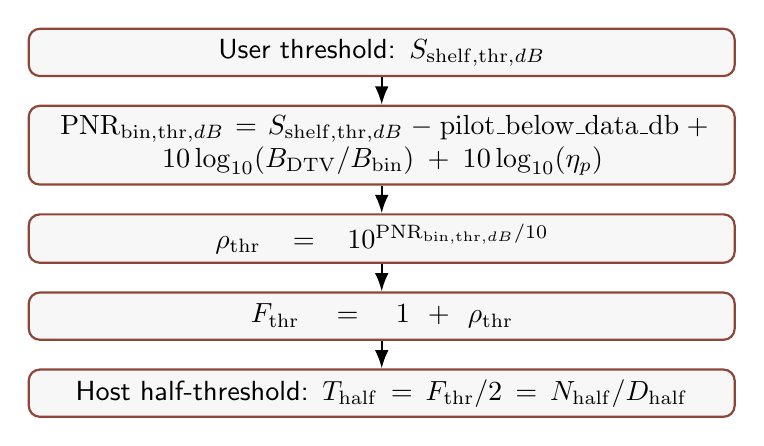
\begin{tikzpicture}[node distance=0.35cm,>=Latex]
\tikzstyle{block}=[rectangle,rounded corners,draw=PilotProxyRed,thick,fill=LightGray,minimum height=0.60cm,text width=0.72\linewidth,align=center]
\node[block] (a) {User threshold: $S_{\mathrm{shelf,thr},dB}$};
\node[block,below=of a] (b) {$\mathrm{PNR}_{\mathrm{bin,thr},dB}=S_{\mathrm{shelf,thr},dB}-\mathrm{pilot\_below\_data\_db}+10\log_{10}(B_{\mathrm{DTV}}/B_{\mathrm{bin}})+10\log_{10}(\eta_p)$};
\node[block,below=of b] (c) {$\rho_{\mathrm{thr}}=10^{\mathrm{PNR}_{\mathrm{bin,thr},dB}/10}$};
\node[block,below=of c] (d) {$F_{\mathrm{thr}}=1+\rho_{\mathrm{thr}}$};
\node[block,below=of d] (e) {Host half-threshold: $T_{\mathrm{half}}=F_{\mathrm{thr}}/2=N_{\mathrm{half}}/D_{\mathrm{half}}$};
\draw[->,thick] (a) -- (b);
\draw[->,thick] (b) -- (c);
\draw[->,thick] (c) -- (d);
\draw[->,thick] (d) -- (e);
\end{tikzpicture}
\caption{Synthetic threshold conversion. The user supplies a shelf-SNR threshold, and the host compares the integer frame powers with a fixed-point rational half-threshold. Here, \(S_{\mathrm{shelf,thr}}\) is the shelf-SNR threshold, \(\eta_p\) is the pilot capture efficiency, \(B_{\mathrm{DTV}}\) and \(B_{\mathrm{bin}}\) are the DTV bandwidth and the bin ENBW, \(\rho_{\mathrm{thr}}\) and \(F_{\mathrm{thr}}\) are the raw excess and the power ratio at threshold, and \(N_{\mathrm{half}}/D_{\mathrm{half}}\) is the rational form of the half-threshold.}
\label{fig:threshold_conversion}
\end{figure}


For a \(-26\dB\) shelf-SNR threshold and the included reference geometry, the checked-in conversion code gives
\begin{lstlisting}[style=shell]
threshold_data_shelf_snr_db       = -26.000
threshold_pilot_excess_db         =  -4.364
threshold_raw_pilot_excess=   0.3661
threshold_coarse_power_ratio          =   1.3661
threshold_half_float         =   0.68305
\end{lstlisting}

The CHIME positive-excess path does not use this user-supplied shelf-SNR
threshold. Int4 quantization makes the target and reference weight norms
slightly unequal, so each weight row has a fixed null point
\begin{equation}
\mu_0=\frac{2\,\lVert w_t\rVert^2}
{\lVert w_{r1}\rVert^2+\lVert w_{r2}\rVert^2}.
\end{equation}
The basic raw convention calls \(F>1\) positive excess. The implementation masks
a valid frame when \(F>\mu_0\), with the inequality evaluated by integer cross
multiplication. We compute \(\mu_0\) from the packed weights, and no mean is
estimated from CANFAR data. This rule corrects the weight-normalization point,
but it supplies neither an empirical false-positive rate nor an operational RFI
severity threshold.

The rule is a recording convention and was not tuned as an operating point. The
rational pair that implements it is per-channel bundle data, and
\field{coarse_power_ratio} is stored for every frame, so a deployment or a later
re-analysis may move the threshold with no kernel change. The adopted Kotekan
deployment moves the decision itself to the fine designated-set CFAR computed
in the kernel. The evaluated alternatives and the first survey calibration are
recorded in the threshold section of the Data Sheet and in
\code{docs/DESIGN_DECISIONS.md}.

\section{Standard and Calibrated Conversion}

The standard synthetic conversion uses
\begin{lstlisting}[style=shell]
--pilot-below-data-db 11.3
--bin-enbw-hz 3051.7578125
--pilot-capture-efficiency 1.0
--dtv-bandwidth-hz 6000000
\end{lstlisting}
The positive field \field{pilot_below_data_db} records how far the pilot power lies below the average data-shelf power. For example, an audit value of \field{measured_pilot_to_data_power_db=-11.9} corresponds to \field{measured_pilot_below_data_db=11.9}.

Calibrated mode is used only when a receiver measurement or model supports the overrides:
\begin{lstlisting}[style=shell]
--pilot-below-data-db VALUE
--bin-enbw-hz VALUE
--pilot-capture-efficiency VALUE
\end{lstlisting}
The output report records the values used, so an analysis can reproduce the conversion.

\section{Fine Products and Interpretation}
\label{sec:fineproducts}

In the time-coherent front end, the windows are integrated coherently after the
dot product, and only the feed sum stays incoherent. The coherent integration gains up to
\ppCoherentGainDb~dB of deflection sensitivity over a reduction that is
incoherent in every step. A per-frame fine spectrum is formed by the kernel
from the exact \code{int32} row sums. First, the rows of each weight term are
reshaped to \([N_{\mathrm{streams}},W]\) windows. The frozen fixed-point FFT
(\code{fxfft256_v1}) is then applied along the window axis with
\(\times\ppFinePadFactor\) zero padding, which gives \ppFineNumBins\ fine bins of
\ppFineBinHz\ Hz. Finally, an incoherent sum over the streams yields the exact
\code{uint64} fine powers \(S_n[b]\) and the fine-bin statistic
\(F_2[b]=2S_t[b]/(S_{r1}[b]+S_{r2}[b])\). The coarse statistic is formed from
the same spectrum. The frame powers are defined as the all-bin sums
\(P_n=\sum_b S_n[b]\), so \(F\) is exactly the all-bin marginal of the fine
spectrum, and no other coarse power path exists. That is, the coarse and fine
statistics come from one set of fine powers. Every product stores both, and the
readers check \(P_n=\sum_b S_n[b]\) exactly. The definitions and stored fields
are given in the Data Sheet and in \code{docs/PRODUCT_SCHEMA.md}, and the CFAR
calibration is stated in \code{docs/METHOD_SPEC.md}.

In CHIME archive products (\code{pilot-proxy chime-scan}), fine products are
mandatory, because the frame powers are their sums. The option \code{--set
fine_products} accepts only \code{on} (the default), and a library without the
row-sum and fine-power entries fails at launch. The only product without fine
terms is that of a pilot out of the measured band
(\field{fine_status=not_applicable_pilot_out_of_band}).

\begin{figure}[H]
\centering
% Shared architecture diagram: detector datapath in the two-stage
% channelizer (filterbank) view.
% Single source of truth -- \input by PilotProxy_DS001 (Data Sheet) and
% PilotProxy_UG001 (User Guide); render detector_datapath.svg for markdown
% use with detector_datapath_standalone.tex. Requires tikz libraries
% arrows.meta + positioning + calc + decorations.pathreplacing, and the
% colors PilotProxyBlue, PilotProxyRed, PilotProxyGray, LightGray from the host document
% (or the standalone wrapper).
% Re-render the svg after editing:
%   cd docs/figures && pdflatex detector_datapath_standalone.tex \
%     && pdftocairo -svg detector_datapath_standalone.pdf detector_datapath.svg
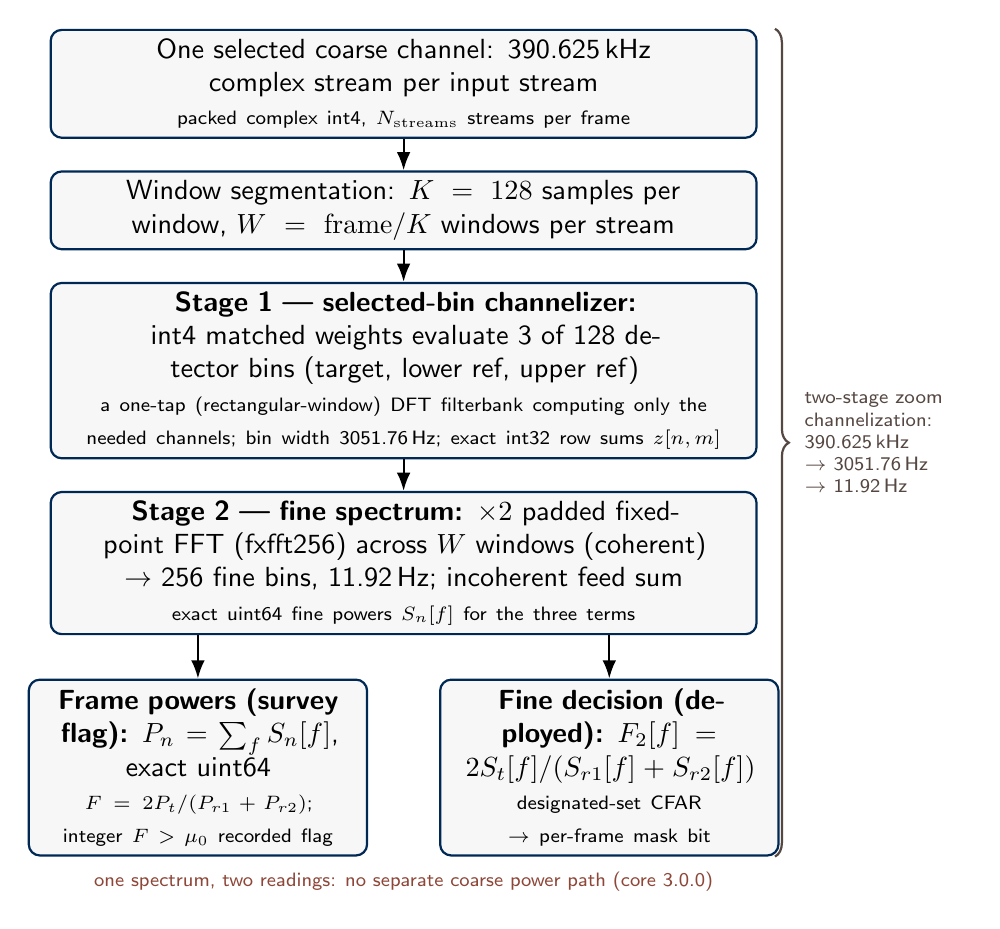
\begin{tikzpicture}[node distance=0.40cm,>=Latex,
  blk/.style={rectangle,rounded corners,draw=PilotProxyBlue,thick,fill=LightGray,
              minimum height=0.62cm,align=center,text width=0.72\linewidth},
  half/.style={rectangle,rounded corners,draw=PilotProxyBlue,thick,fill=LightGray,
               minimum height=0.62cm,align=center,text width=0.335\linewidth}]

\node[blk] (in) {One selected coarse channel: 390.625\,kHz complex stream
  per input stream\\ \scriptsize packed complex int4,
  $N_{\mathrm{streams}}$ streams per frame};
\node[blk,below=of in] (seg) {Window segmentation: $K=128$ samples per
  window, $W=\mathrm{frame}/K$ windows per stream};
\node[blk,below=of seg] (s1) {\textbf{Stage 1 --- selected-bin
  channelizer:} int4 matched weights evaluate 3 of 128 detector bins
  (target, lower ref, upper ref)\\ \scriptsize a one-tap
  (rectangular-window) DFT filterbank computing only the needed channels;
  bin width 3051.76\,Hz; exact int32 row sums $z[n,m]$};
\node[blk,below=of s1] (s2) {\textbf{Stage 2 --- fine spectrum:}
  $\times 2$ padded fixed-point FFT (fxfft256) across $W$ windows
  (coherent) $\to$ 256 fine bins, 11.92\,Hz; incoherent feed sum\\
  \scriptsize exact uint64 fine powers $S_n[f]$ for the three terms};
\node[half,anchor=north east] (v1) at ($(s2.south)+(-0.45,-0.55)$)
  {\textbf{Frame powers (survey flag):} $P_n=\sum_f S_n[f]$, exact
  uint64\\ \scriptsize $F = 2P_t/(P_{r1}+P_{r2})$; integer $F>\mu_0$
  recorded flag};
\node[half,anchor=north west] (v2) at ($(s2.south)+(0.45,-0.55)$)
  {\textbf{Fine decision (deployed):}
  $F_2[f]=2S_t[f]/(S_{r1}[f]+S_{r2}[f])$\\
  \scriptsize designated-set CFAR $\to$ per-frame mask bit};

\draw[->,thick] (in) -- (seg);
\draw[->,thick] (seg) -- (s1);
\draw[->,thick] (s1) -- (s2);
\draw[->,thick] (s2.south -| v1.north) -- (v1.north);
\draw[->,thick] (s2.south -| v2.north) -- (v2.north);
\node[font=\scriptsize\color{PilotProxyRed},align=center]
  at ($(s2.south |- v2.south)+(0,-0.32)$)
  {one spectrum, two readings: no separate coarse power path (core 3.0.0)};

\coordinate (brx) at ([xshift=0.22cm]s1.east);
\draw[decorate,decoration={brace,amplitude=5pt},thick,PilotProxyGray]
  (brx |- in.north) -- (brx |- v2.south)
  node[midway,right=7pt,font=\scriptsize\color{PilotProxyGray},align=left,
       text width=2.0cm]
  {two-stage zoom channelization:\\ 390.625\,kHz\\ $\to$ 3051.76\,Hz\\
   $\to$ 11.92\,Hz};
\end{tikzpicture}

\caption{Detector datapath drawn as a filterbank. Stage 1 is a selected-bin DFT
filterbank that produces the detector bins, and stage 2 is the padded
window-axis FFT that produces the fine bins. The two stages form a standard
two-stage zoom channelization that computes only the channels the detector
needs.}
\label{fig:detector_datapath}
\end{figure}

In the products, designated bin 0 is the nominal ATSC pilot. A real transmitter
is rarely exactly there. Full-power stations hold a \(\pm1\) kHz tolerance, and
translator-class stations have no specified tolerance. A genuine pilot
therefore typically appears as a persistent detected line at a fixed nonzero
offset in the fine span (half a detector bin on either side of nominal), and
the designated bin itself may rarely fire. The any-bin decision rule exists for
this case. Two consequences follow. First, a transmitter is recognized by the
stability of its offset over frames and epochs, and designated-bin hits are a
poor guide. Second, on DTV-occupied channels the offset pilot lies in
non-designated bins, so \field{fine_null_bulk_exceedance_fraction} can be high
there. This field is the in-sample fraction of fitted null-bulk bins above the
fitted threshold, and it is not an independently measured false-alarm rate. It
is read together with the stored fine spectrum and the stability of the
detected line over frames.

\section{C API Overview}

The public C API is declared in \code{cuda/pilotproxy_detector.h}. In this example, \code{d_in}, \code{d_fine_power_out}, and \code{d_power_out} are device pointers, and \code{host_weights} is a host pointer. A typical measurement call is
\begin{lstlisting}[style=cstyle,language=C]
int K, N, bits, ref_offset;
PilotProxy_GetSpecs(&K, &N, &bits, &ref_offset);

void* h = PilotProxy_Create(d_in, detector_rows_per_block);
if (h == NULL) {
    /* Read PilotProxy_LastError() and stop. */
    return;
}
PilotProxy_Compute_FusedFine_U64(
    h,
    host_weights,
    d_fine_power_out,   /* batch * N * 256 uint64: S_n[b] */
    d_power_out,        /* batch * N uint64: P_n = sum_b S_n[b] */
    NULL);              /* optional int32 row-sum debug tap */
if (PilotProxy_LastError()[0] != 0) {
    /* Handle the recorded CUDA/API error. */
}
PilotProxy_Destroy(h);
\end{lstlisting}
The compute call writes the three frame powers
\begin{equation}
  \mathrm{d\_power\_out}=(P_t,\;P_{r1},\;P_{r2}),\qquad P_n=\sum_b S_n[b],
\end{equation}
and host code then computes
\begin{equation}
  F=\frac{2P_t}{P_{r1}+P_{r2}}
\end{equation}
and the norm-corrected mask in exact integer arithmetic, so the library forms no
ratio and no coarse mask. \(F\) is undefined for a zero denominator. In that
case, the host marks the frame invalid and forces its mask to zero, so Python
callers must inspect \field{p_ref_sum_u64} (or \field{valid}) before they
interpret any conversion. The deployed mask bit comes from
\apicode{PilotProxy_Compute_FusedFineMask_U64} or
\apicode{PilotProxy_Compute_FusedFineMaskWithSupport_U64}.

A capability probe guards the row-sum entry:
\begin{lstlisting}[style=cstyle,language=C]
if (PilotProxy_Supports_RowSums()) {
    /* d_matched_filter_row_projections_out: device int32, batch * N * rows * 2 elements
       (term-major, stream-major rows, interleaved re/im). */
    PilotProxy_Compute_RowSums_I32(h, host_weights, d_matched_filter_row_projections_out);
}
\end{lstlisting}
The values are exact integers and are the input of
\apicode{PilotProxy_Compute_FinePowers_U64}. In the staged path, the fine powers
of that stage are summed over bins on the host, and the frame powers obtained
are bit for bit the same as those of the fused entry. Rows keep the
stream-major order of the packer, so a term slice reshapes to
\code{[num_streams, windows_per_stream]} with no gather.

In deployment, only the per-frame \code{mask} (1 = reject) crosses the proposed
interface, and the fine-power, frame-power, and row-sum readbacks feed the
archive science products and diagnostics.

\section{JSON Output Policy}

JSON reports emit no NaN or infinity, and values that are not finite are serialized as \code{null}. CSV files may keep NaN text when the analysis software can represent it.

Detector and synthetic SNR-evaluator JSON reports carry \field{result_schema} with \code{schema_version=pilotproxy_result_schema_v2}. This object records the statistic definition, layout, calibration constants, threshold conversion, fixed-point contract, and mask convention needed to interpret those reports. Audit, quantization, summary, injection, and CHIME products use their own documented top-level schemas. CHIME per-pilot archive products, for example, use \field{schema_version}=\texttt{\ppPerPilotSchema} as defined in \code{docs/PRODUCT_SCHEMA.md}.

The statistic over summed blocks is:
\begin{equation}
F = \frac{2\sum_r P_{t,r}}{\sum_r P_{r1,r}+\sum_r P_{r2,r}},
\end{equation}
where \(r\) indexes the summed blocks and each \(P_{n,r}\) is a frame power,
the all-bin sum of that block's fine powers. We sum powers first and form one
ratio, since an average of per-block power ratios would define a different
estimator.

When a product averages masked data, rejected blocks are excluded from both the
sum and the count, and no zero is filled in their place:
\begin{equation}
\bar{P}_{\mathrm{after}} =
\frac{\sum_b P_b(1-M_b)}{\sum_b (1-M_b)}.
\end{equation}
Here, \(M_b=1\) excludes block \(b\).

\section{Result Summaries}

The summary helper reduces a result file to compact CSV and JSON statistics:
\begin{lstlisting}[style=shell]
pilot-proxy summarize-results \
  --input generated/dtv_snr_eval/dtv_snr_eval.json \
  --output-dir generated/summary
\end{lstlisting}
This command writes \code{summary.csv} and \code{summary.json}. For an SNR
sweep, histograms are skipped, because the input mixes populations at different
requested SNRs. A histogram is easier to interpret for repeated trials at one
fixed SNR, and \code{--histograms always} is used only when the mixed
distribution is meant to be part of the diagnostic.

\section{Known Limitations}

\begin{itemize}
  \item The synthetic testbench models GNU Radio ATSC 1.0 signals only. Other broadcast standards and telescope performance are not covered.
  \item The CHIME real-data workflow (\code{chime-run}, \code{chime-scan}, and the HDF5 reader) is documented in \code{docs/CANFAR_RUNBOOK.md} and \code{docs/CHIME_RUN_WORKFLOW.md}.
  \item The checked-in CHIME profile and stream map must still agree with the data product being processed. The 16384-sample frame is the planned F-engine upgrade profile used by this repository and makes no claim about the frame deployed today. \code{chime-run} uses its explicit override, and \code{chime-scan} uses the Pilot Proxy CHIME instrument \code{nfft}. Neither path discovers a universal HDF5 frame size.
  \item Synthetic threshold tests accept a shelf-SNR threshold, while the CHIME path uses $F>\mu_0$, with \(\mu_0\) fixed by the weight norms. Neither rule is a telescope false-positive threshold calibrated on data.
  \item Receiver profiles define an adapter contract. A profile does not show that a telescope pipeline has been deployed or validated.
  \item Installed packages carry the weight bank and \code{configs/} resources, so default-resource commands can run from any directory. Repository-relative examples, helper scripts, second-interpreter subprocesses, and the CUDA build require a checkout or explicit paths. The CUDA kernel itself is not packaged and builds from the cloned source tree (\code{make build-kernel}).
  \item Fine products are mandatory, because the frame powers are their all-bin sums. A library without the row-sum and fine-power entries fails at launch, and \code{fine_products} accepts only \code{on}.
\end{itemize}

\section{Troubleshooting}

\subsection{GNU Radio imports fail}
The system GNU Radio Python, typically \code{/usr/bin/python3}, must be able to import PilotProxy from the editable checkout or through an explicit \code{PYTHONPATH}. A wheel installed only in the CUDA environment is not visible to it. \code{PYTHONNOUSERSITE=1} is set when user-site packages shadow the GNU Radio NumPy build.

\subsection{CUDA shared library not found}
The library is rebuilt with \code{make build-kernel SM=<target>}, and \code{LD_LIBRARY_PATH} must hold the CUDA driver path. On WSL, this path is commonly \code{/usr/lib/wsl/lib}, and it is verified on the target host. The staged cache copy under \code{~/.cache/pilot_proxy/} is preferred.

\subsection{Wrong detector matrix shape}
The packed detector matrix must have dtype \code{int8} and last dimension equal
to the selected compiled detector window (64 or 128). \code{pilot-proxy quantize}
builds the expected format.

\subsection{No weights for channel}
The shipped bank covers physical channels 14 through 36, and \code{pilot-proxy list-channels} lists the available targets.

\subsection{PNR is null}
If \(F\leq1\), the raw pilot-excess ratio is non-positive and \(10\log_{10}(F-1)\) is undefined. The JSON value is therefore \code{null}, which can occur for noise-only and weak-signal trials.

\subsection{A scan fails at launch for want of fine powers}
The loaded \code{libpilotproxy.so} lacks the row-sum or fine-power entry, or it
is from another core major. The library is rebuilt and restaged with
\code{make build-kernel}, \code{PilotProxy_Supports_RowSums()} and
\code{PilotProxy_Supports_FinePowers()} are confirmed to return 1 (the
kernel-load check in \code{scripts/setup_env.sh} prints the loaded version), and
the scan is relaunched. No degraded mode exists, because the frame powers are
the sums of the fine powers.

\subsection{High null-bulk exceedance fraction on an occupied channel}
\field{fine_null_bulk_exceedance_fraction} counts detections in non-designated bins. A real transmitter at a nonzero pilot offset occupies those bins persistently, so a high fraction on a DTV-occupied channel is the expected signal (see Section~\ref{sec:fineproducts}). The CFAR calibration is evaluated on channels without detected lines.

\begin{thebibliography}{9}
\bibitem{atsc_a53_part2_2011} Advanced Television Systems Committee, \emph{ATSC Digital Television Standard, Part 2: RF/Transmission System Characteristics}, A/53 Part 2:2011, 15 December 2011. \url{https://www.atsc.org/wp-content/uploads/2021/04/A53-Part-2-2011.pdf}
\bibitem{ecfr_73603} Electronic Code of Federal Regulations, 47 CFR \S 73.603, \emph{Numerical designation of television channels}. \url{https://www.ecfr.gov/current/title-47/chapter-I/subchapter-C/part-73/subpart-E/section-73.603}
\bibitem{gnuradio_dtv} GNU Radio Manual, \emph{DTV/ATSC module documentation}. \url{https://www.gnuradio.org/doc/sphinx-3.7.7.1/atsc/index.html}
\bibitem{gnuradio_noise} GNU Radio Manual, \emph{gr::analog::noise\_source}, complex noise-source amplitude convention. \url{https://www.gnuradio.org/doc/doxygen/classgr_1_1analog_1_1noise__source.html}
\end{thebibliography}

\end{document}
